\begin{frame}
    \titlepage
\end{frame}

\begin{frame}
    \frametitle{Introduction}
    \begin{itemize}
        \item \textbf{Significance of Breast Cancer as a Global Health Issue}
              \begin{itemize}
                  \item In 2022, approximately \textbf{2.3 million women} were diagnosed with breast cancer worldwide.
                  \item This represents about \textbf{one in four} of all cancers in women.
                  \item In 2022, \textbf{670,000 women} died from breast cancer worldwide.
                  \item In 2020, breast cancer was the cause of \textbf{16\%} of cancer deaths in women.
                  \item Breast cancer incidence has increased by more than \textbf{20\%} since 2008.
                  \item Breast cancer incidence is growing in many parts of the world, especially in transitioning countries.
                  \item In 2019, \textbf{25,100 men} were diagnosed with breast cancer globally.
              \end{itemize}
    \end{itemize}
\end{frame}

\begin{frame}
    \frametitle{Breast Cancer Overview Image}
    \begin{center}
        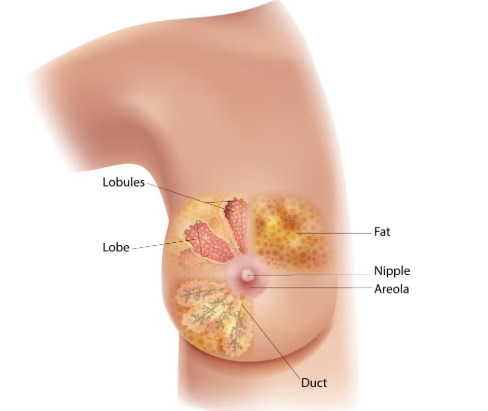
\includegraphics[width=1\textwidth]{images/breastimage.png}
    \end{center}
\end{frame}

\begin{frame}
    \frametitle{Brief intro to types of breast cancer}

    \textbf{Benign vs. Malignant Tumors}
    \begin{center}
        \begin{tabular}{ | >{\bfseries}l | >{\raggedright\arraybackslash}p{5cm} | }
            \hline
            \textbf{Category}         & \textbf{Description}                                                                                               \\
            \hline
            \textbf{Benign Tumors}    & Non-cancerous, usually slow-growing, doesn't spread, usually not life-threatening.                                 \\
            \hline
            \textbf{Malignant Tumors} & Cancerous, can grow rapidly, invade surrounding tissues, spread to other body parts, potentially life-threatening. \\
            \hline
        \end{tabular}
    \end{center}
\end{frame}

\begin{frame}
    \frametitle{Brief intro to types of breast cancer}

    \textbf{Invasive Breast Cancers: Types}
    \begin{center}
        \begin{tabular}{ | >{\bfseries}l | >{\raggedright\arraybackslash}p{4cm} | >{\raggedright\arraybackslash}p{4cm} | }
            \hline
            \textbf{Feature}      & \textbf{Invasive Ductal Carcinoma (IDC)}         & \textbf{Invasive Lobular Carcinoma (ILC)}                                            \\
            \hline
            \textbf{Frequency}    & Most common type of breast cancer (70-80\%).     & Second most common (10-15\%).                                                        \\
            \hline
            \textbf{Origin}       & Starts in the milk ducts.                        & Starts in the milk lobules.                                                          \\
            \hline
            \textbf{Presentation} & May form a lump and may spread to other tissues. & May not typically form a lump; presents as a thickening and may affect both breasts. \\
            \hline
        \end{tabular}
    \end{center}
\end{frame}

\begin{frame}
    \frametitle{Project Motivation}
    {\LARGE
        \begin{itemize}
            \item Chose this topic because breast cancer is a major issue.
            \item Goals of the project:
                  \begin{itemize}
                      \item Analyze key datasets related to breast cancer.
                      \item Apply statistical methods to uncover significant insights.
                      \item Inform strategies for early detection and treatment.
                  \end{itemize}
        \end{itemize}
    }
\end{frame}

\begin{frame}
    \frametitle{Dataset Introduction}
    \textbf{Source of the Dataset:}\\[1ex]
    This breast cancer domain was obtained from the University Medical Centre, Institute of Oncology, Ljubljana, Yugoslavia. This is one of three domains provided by the Oncology Institute that has repeatedly appeared in the machine learning literature.
    
    \vspace{1em}
    \textbf{Citations:}\\[0.5ex]
    Zwitter, M. \& Soklic, M. (1988). Breast Cancer [Dataset]. UCI Machine Learning Repository. \href{https://doi.org/10.24432/C51P4M}{https://doi.org/10.24432/C51P4M}
    
    \vspace{1em}
    \textbf{Download Link:}\\[0.5ex]
    \href{https://archive.ics.uci.edu/dataset/14/breast+cancer}{https://archive.ics.uci.edu/dataset/14/breast+cancer}
    \href{https://data.worldbank.org/indicator/NY.GDP.MKTP.CD}{Global GDP indicators}
\end{frame}


\begin{frame}
    \frametitle{Breast Cancer Statistics by Country Preview}
    \input{tables/breast_country_sample_part1.tex}
    \vspace{1em}
    \input{tables/breast_country_sample_part2.tex}
\end{frame}

\begin{frame}
    \frametitle{Statistical Measures and Tools - Introduction}
    \textbf{Statistical Tools for Data Analysis}

    In this section, we will introduce the statistical measures, concepts, and visualization tools employed to analyze the breast cancer datasets. These tools help us to:
    \vspace{1em}
    \begin{itemize}
        \item Identify patterns
        \item Make sense of the data
        \item Extrapolate meanings and trends
    \end{itemize}
\end{frame}

\begin{frame}
    \frametitle{Statistical Measures and Tools (Part 1)}
    \textbf{Categories of Statistical Tools Used: Descriptive Statistics (Part 1)}
    \begin{columns}
        \begin{column}{0.5\textwidth}
            \begin{itemize}
                \item Mean
                \item Median
                \item Mode
                \item Minimum/S
                \item Maximum/L
                \item Range
                \item Coefficient of Range
                \item MD Mean
                \item MD Median
            \end{itemize}
        \end{column}
        \begin{column}{0.5\textwidth}
            \begin{itemize}
                \item Standard Deviation
                \item Variance
                \item Coefficient of SD
                \item CV
                \item IQR
                \item QD
                \item Midrange
                \item Quartiles ($Q_1, Q_2, Q_3$)
                \item Deciles ($D_1$ to $D_9$)
                \item Percentiles ($P_1$ to $P_{99}$)
            \end{itemize}
        \end{column}
    \end{columns}
\end{frame}

\begin{frame}
    \frametitle{Statistical Measures and Tools (Part 2)}
    \textbf{Categories of Statistical Tools Used: Statistical Formulas}
    \begin{columns}
        \begin{column}{0.5\textwidth}
            \begin{itemize}
                \item Central Moments ($\mu_r$)
                \item Raw Moments ($\mu'_r$)
                \item Skewness (Moments)
                \item Kurtosis (Percentiles)
                \item Excess Kurtosis (Moments)
                \item Covariance
                \item Pearson Skewness
            \end{itemize}
        \end{column}
        \begin{column}{0.5\textwidth}
            \begin{itemize}
                \item Bowley Skewness
                \item Correlation
                \item Regression byx ($b_{yx}$)
                \item Regression bxy ($b_{xy}$)
                \item Chebyshev's Inequality
                \item Normal PDF
            \end{itemize}
        \end{column}
    \end{columns}
\end{frame}

\begin{frame}
    \frametitle{Statistical Measures and Tools (Part 3)}
    \textbf{Categories of Statistical Tools Used:}
    \begin{columns}
        \begin{column}{0.5\textwidth}
            \textbf{Statistical Concepts and Tools}
            \begin{itemize}
                \item PMF
                \item PDF
                \item CDF
                \item Expected Value
                \item Variance
                \item R-squared
            \end{itemize}
            \vspace{1em}
            \textbf{Inferential Statistics}
            \begin{itemize}
                \item Regression Analysis
            \end{itemize}
        \end{column}
        \begin{column}{0.5\textwidth}
            \textbf{Visualization tools}
            \begin{itemize}
                \item Histogram
                \item Boxplots
                \item Sorted Bar Graph
                \item Normal graph
                \item Scatter plot
                \item Q-Q plot (Quantile-quantile plot)
                \item Correlation Heatmap
            \end{itemize}
        \end{column}
    \end{columns}
\end{frame}